% !TEX TS-program = pdflatex
\documentclass[11pt]{article}

% -------------------- Packages --------------------
\usepackage[a4paper,margin=1in]{geometry}
\usepackage{amsmath,amssymb}
\usepackage[T1]{fontenc}
\usepackage{lmodern}
\usepackage{xcolor}
\usepackage{tcolorbox}
\tcbuselibrary{skins,breakable}
\usepackage{enumitem}
\usepackage{hyperref}
\usepackage{tikz}
\usetikzlibrary{calc,angles,quotes,shapes.geometric}

\pagestyle{empty}

% -------------------- Dark Theme Colors --------------------
\definecolor{bg}{HTML}{000000}
\definecolor{pairbg}{HTML}{121212}
\definecolor{solbg}{HTML}{0A0A0A}
\definecolor{border}{HTML}{2A2A2A}
\definecolor{text}{HTML}{FFFFFF}
\definecolor{muted}{HTML}{C9CDD3}
\definecolor{gold}{HTML}{FFD700}
\definecolor{green}{HTML}{4ADE80}
\definecolor{cyan}{HTML}{38BDF8}

\pagecolor{bg}
\color{text}

\hypersetup{
  colorlinks=true,
  linkcolor=cyan,
  urlcolor=cyan
}

\setlength{\parindent}{0pt}
\setlength{\parskip}{10pt}

\setlist[itemize]{left=1.4em,itemsep=6pt,topsep=6pt}
\setlist[enumerate]{left=1.6em,itemsep=4pt,topsep=4pt}

% -------------------- tcolorbox Base --------------------
\tcbset{
  enhanced,
  breakable,
  arc=12pt,
  boxrule=0.8pt,
  left=16pt,right=16pt,top=12pt,bottom=12pt
}

\newtcolorbox{QAPair}[1]{%
  colback=pairbg,
  colbacklower=solbg,
  colframe=border,
  coltext=text,
  title=\textcolor{gold}{\bfseries #1},
  fonttitle=\bfseries,
  coltitle=text,
  segmentation style={draw=border, dashed, line width=0.6pt},
}

\newtcolorbox{QuickBox}{%
  colback=pairbg,
  colframe=cyan,
  coltext=text,
  fontupper=\color{text},
  borderline north={4pt}{0pt}{cyan},
  arc=14pt,
  boxrule=0.8pt
}

% Helper for step headings
\newcommand{\Step}[1]{\textcolor{muted}{\textbf{Step #1:}}}

% Helper (TikZ style)
\tikzset{
  lab/.style={text=text, font=\small},
  dim/.style={text=cyan, font=\small},
  shapeLine/.style={line width=1pt, draw=cyan},
  shapeFill/.style={fill=cyan!20, draw=cyan, line width=1pt},
  ball/.style={shade, ball color=cyan!20, draw=cyan}
}

% ============================================================
\begin{document}

\begin{center}
{\LARGE\bfseries \textcolor{gold}{Exercise 9.3 --- Solutions}}\\[-2pt]
\end{center}

\begin{QuickBox}
{\color{cyan}\bfseries Quick formulas (Similarity)}\par\medskip
\begin{itemize}
\item \textbf{Similar figures:} corresponding \textbf{length ratio} is constant ($k$).
\item \textbf{Area scale:} if length scale is $k$, then \;\;$\dfrac{A_2}{A_1}=k^2$.
\item \textbf{Surface area of similar 3D shapes:} also scales as $k^2$.
\item \textbf{From areas to lengths:} \;\;$k=\sqrt{\dfrac{A_2}{A_1}}$.
\end{itemize}
\end{QuickBox}

% ============================================================
% Q1
\begin{QAPair}{Question 1 (i)}
\textcolor{gold}{\bfseries Question:} Two similar right triangles have corresponding heights $4$ cm and $6$ cm.
If the larger has area $A_2=36\text{ cm}^2$, find $A_1$.

\begin{center}
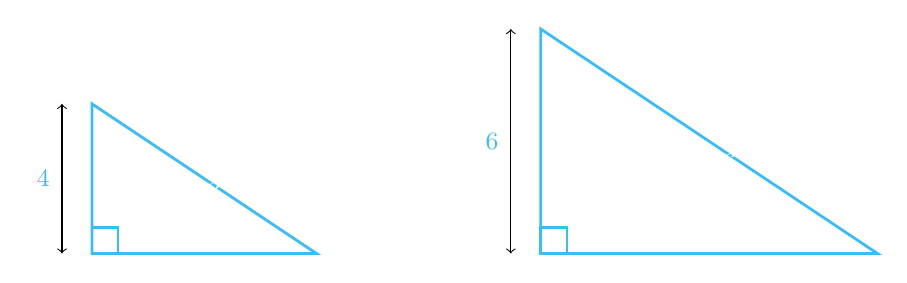
\begin{tikzpicture}[scale=0.95]
% small triangle
\coordinate (A) at (0,0);
\coordinate (B) at (0,2);
\coordinate (C) at (3,0);
\draw[shapeLine] (A)--(B)--(C)--cycle;
\draw[shapeLine] (A) rectangle +(0.35,0.35);
\node[lab] at (1.25,0.8) {$A_1=?$};
\draw[<->,dim] (-0.4,0) -- (-0.4,2);
\node[dim] at (-0.65,1) {$4$};

% large triangle
\begin{scope}[xshift=6cm]
\coordinate (A2) at (0,0);
\coordinate (B2) at (0,3);
\coordinate (C2) at (4.5,0);
\draw[shapeLine] (A2)--(B2)--(C2)--cycle;
\draw[shapeLine] (A2) rectangle +(0.35,0.35);
\node[lab] at (2.0,1.2) {$A_2=36$};
\draw[<->,dim] (-0.4,0) -- (-0.4,3);
\node[dim] at (-0.65,1.5) {$6$};
\end{scope}
\end{tikzpicture}
\end{center}

\tcblower
\textcolor{green}{\bfseries Answer:}
\[
\begin{aligned}
\Step{1}\;& \text{Length scale }k=\frac{4}{6}=\frac{2}{3}.\\
\Step{2}\;& \frac{A_1}{A_2}=k^2=\left(\frac{2}{3}\right)^2=\frac{4}{9}.\\
\Step{3}\;& A_1=36\cdot \frac{4}{9}=16.
\end{aligned}
\]
\[
\boxed{A_1=16\text{ cm}^2}
\]
\end{QAPair}

\begin{QAPair}{Question 1 (ii)}
\textcolor{gold}{\bfseries Question:} Two similar rectangles have corresponding lengths $9$ cm and $4$ cm.
If $A_1=162\text{ cm}^2$, find $A_2$.

\begin{center}
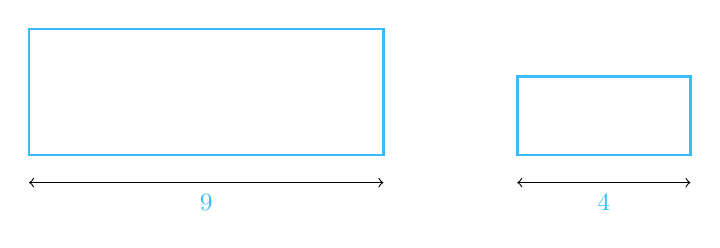
\begin{tikzpicture}[scale=1.0]
\draw[shapeLine] (0,0) rectangle (4.5,1.6);
\node[lab] at (2.25,0.8) {$A_1=162$};
\draw[<->,dim] (0,-0.35)--(4.5,-0.35);
\node[dim] at (2.25,-0.6) {$9$};

\begin{scope}[xshift=6.2cm]
\draw[shapeLine] (0,0) rectangle (2.2,1.0);
\node[lab] at (1.1,0.5) {$A_2=?$};
\draw[<->,dim] (0,-0.35)--(2.2,-0.35);
\node[dim] at (1.1,-0.6) {$4$};
\end{scope}
\end{tikzpicture}
\end{center}

\tcblower
\textcolor{green}{\bfseries Answer:}
\[
\begin{aligned}
\Step{1}\;& k=\frac{4}{9}.\\
\Step{2}\;& \frac{A_2}{A_1}=k^2=\left(\frac{4}{9}\right)^2=\frac{16}{81}.\\
\Step{3}\;& A_2=162\cdot \frac{16}{81}=32.
\end{aligned}
\]
\[
\boxed{A_2=32\text{ cm}^2}
\]
\end{QAPair}

\begin{QAPair}{Question 1 (iii)}
\textcolor{gold}{\bfseries Question:} Two similar trapeziums have corresponding top sides $3$ cm and $6$ cm.
If $A_2=996\text{ cm}^2$, find $A_1$.

\begin{center}
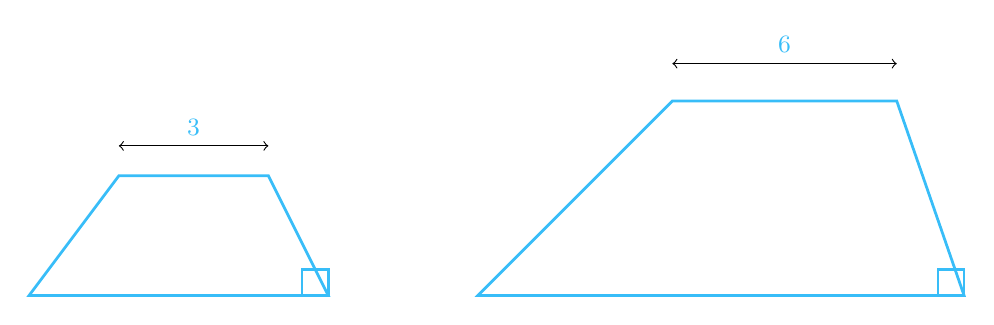
\begin{tikzpicture}[scale=0.95]
% small trapezium
\coordinate (P) at (0,0);
\coordinate (Q) at (4,0);
\coordinate (R) at (3.2,1.6);
\coordinate (S) at (1.2,1.6);
\draw[shapeLine] (P)--(Q)--(R)--(S)--cycle;
\draw[shapeLine] (Q) rectangle +(-0.35,0.35);
\node[lab] at (2.2,0.8) {$A_1=?$};
\draw[<->,dim] (1.2,2.0)--(3.2,2.0);
\node[dim] at (2.2,2.25) {$3$};

% large trapezium
\begin{scope}[xshift=6.0cm]
\coordinate (P2) at (0,0);
\coordinate (Q2) at (6.5,0);
\coordinate (R2) at (5.6,2.6);
\coordinate (S2) at (2.6,2.6);
\draw[shapeLine] (P2)--(Q2)--(R2)--(S2)--cycle;
\draw[shapeLine] (Q2) rectangle +(-0.35,0.35);
\node[lab] at (3.5,1.2) {$A_2=996$};
\draw[<->,dim] (2.6,3.1)--(5.6,3.1);
\node[dim] at (4.1,3.35) {$6$};
\end{scope}
\end{tikzpicture}
\end{center}

\tcblower
\textcolor{green}{\bfseries Answer:}
\[
\begin{aligned}
\Step{1}\;& k=\frac{3}{6}=\frac12.\\
\Step{2}\;& A_1=A_2\cdot k^2=996\cdot \left(\frac12\right)^2=996\cdot \frac14=249.
\end{aligned}
\]
\[
\boxed{A_1=249\text{ cm}^2}
\]
\end{QAPair}

\begin{QAPair}{Question 1 (iv)}
\textcolor{gold}{\bfseries Question:} Two similar circles have radii $3.6$ cm and $1.8$ cm.
If $A_1=180\text{ cm}^2$, find $A_2$.

\begin{center}
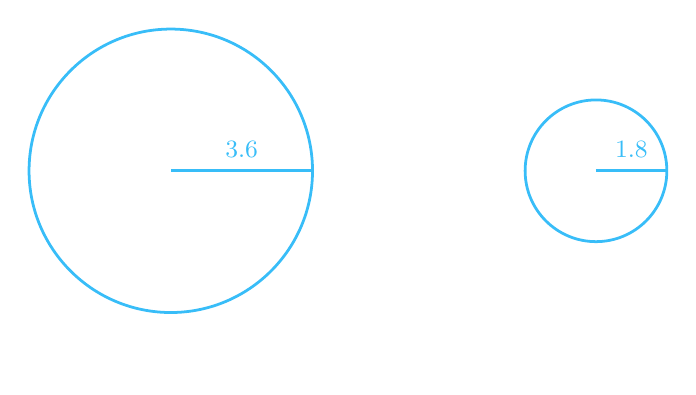
\begin{tikzpicture}[scale=0.9]
\draw[shapeLine] (0,0) circle (2.0);
\draw[shapeLine] (0,0)--(2.0,0);
\node[dim] at (1.0,0.3) {$3.6$};
\node[lab] at (0,-2.5) {$A_1=180$};

\begin{scope}[xshift=6cm]
\draw[shapeLine] (0,0) circle (1.0);
\draw[shapeLine] (0,0)--(1.0,0);
\node[dim] at (0.5,0.3) {$1.8$};
\node[lab] at (0,-1.7) {$A_2=?$};
\end{scope}
\end{tikzpicture}
\end{center}

\tcblower
\textcolor{green}{\bfseries Answer:}
\[
\begin{aligned}
\Step{1}\;& k=\frac{1.8}{3.6}=\frac12.\\
\Step{2}\;& A_2=A_1\cdot k^2=180\cdot \left(\frac12\right)^2=180\cdot \frac14=45.
\end{aligned}
\]
\[
\boxed{A_2=45\text{ cm}^2}
\]
\end{QAPair}

% ============================================================
% Q2
\begin{QAPair}{Question 2 (i)}
\textcolor{gold}{\bfseries Question:} Two similar triangles have areas $A_1=12\text{ cm}^2$ and $A_2=108\text{ cm}^2$.
If the smaller base is $2$ cm, find the larger base $x$.

\begin{center}
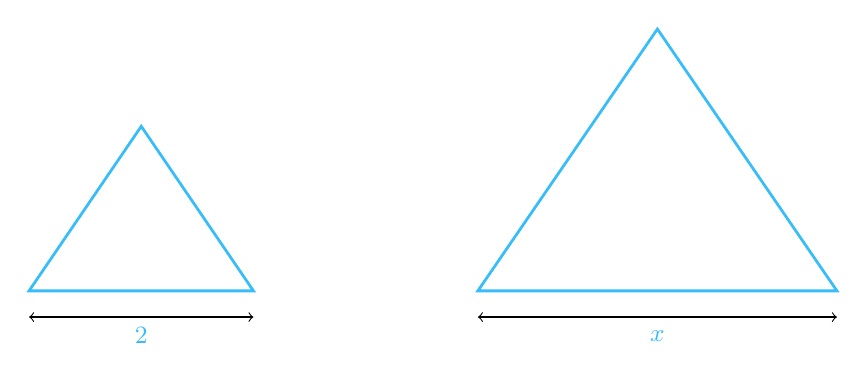
\begin{tikzpicture}[scale=0.95]
\draw[shapeLine] (0,0)--(1.5,2.2)--(3,0)--cycle;
\node[lab] at (1.5,0.9) {$A_1=12$};
\draw[<->,dim] (0,-0.35)--(3,-0.35);
\node[dim] at (1.5,-0.6) {$2$};

\begin{scope}[xshift=6cm]
\draw[shapeLine] (0,0)--(2.4,3.5)--(4.8,0)--cycle;
\node[lab] at (2.4,1.3) {$A_2=108$};
\draw[<->,dim] (0,-0.35)--(4.8,-0.35);
\node[dim] at (2.4,-0.6) {$x$};
\end{scope}
\end{tikzpicture}
\end{center}

\tcblower
\textcolor{green}{\bfseries Answer:}
\[
\begin{aligned}
\Step{1}\;& \frac{A_2}{A_1}=\frac{108}{12}=9.\\
\Step{2}\;& k=\sqrt{9}=3 \quad (\text{length scale}).\\
\Step{3}\;& x=2\cdot 3=6.
\end{aligned}
\]
\[
\boxed{x=6\text{ cm}}
\]
\end{QAPair}

\begin{QAPair}{Question 2 (ii)}
\textcolor{gold}{\bfseries Question:} Two similar parallelograms have areas $A_1=50\text{ cm}^2$ and $A_2=200\text{ cm}^2$.
If the corresponding side of the larger is $10$ cm, find $x$ for the smaller.

\begin{center}
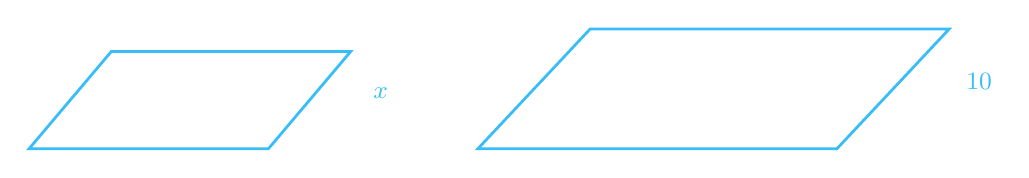
\begin{tikzpicture}[scale=0.95]
% small parallelogram
\draw[shapeLine] (0,0)--(3.2,0)--(4.3,1.3)--(1.1,1.3)--cycle;
\node[lab] at (2.2,0.7) {$A_1=50$};
\node[dim] at (4.7,0.75) {$x$};

% large parallelogram
\begin{scope}[xshift=6cm]
\draw[shapeLine] (0,0)--(4.8,0)--(6.3,1.6)--(1.5,1.6)--cycle;
\node[lab] at (3.2,0.85) {$A_2=200$};
\node[dim] at (6.7,0.9) {$10$};
\end{scope}
\end{tikzpicture}
\end{center}

\tcblower
\textcolor{green}{\bfseries Answer:}
\[
\begin{aligned}
\Step{1}\;& \frac{A_2}{A_1}=\frac{200}{50}=4.\\
\Step{2}\;& k=\sqrt{4}=2.\\
\Step{3}\;& 10 = 2x \;\Rightarrow\; x=5.
\end{aligned}
\]
\[
\boxed{x=5\text{ cm}}
\]
\end{QAPair}

\begin{QAPair}{Question 2 (iii)}
\textcolor{gold}{\bfseries Question:} Two similar cone-like figures have areas $A_1=900\text{ cm}^2$ and $A_2=100\text{ cm}^2$.
If the corresponding length of the smaller is $10$ cm, find $x$ for the larger.

\begin{center}
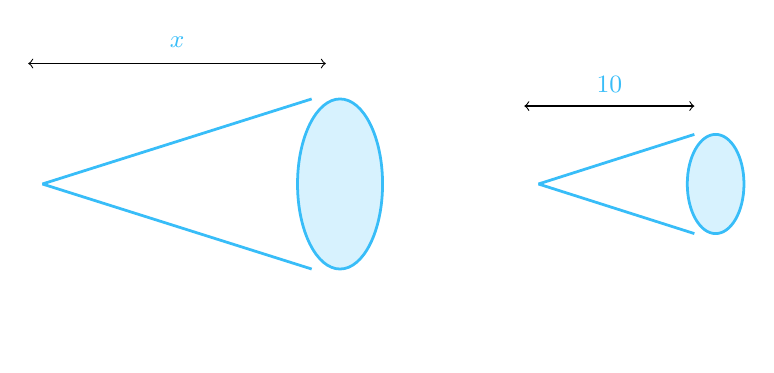
\begin{tikzpicture}[scale=0.9]
% larger
\coordinate (V1) at (0,0);
\draw[shapeLine] (V1)--(3.8,1.2);
\draw[shapeLine] (V1)--(3.8,-1.2);
\draw[shapeFill] (4.2,0) ellipse (0.6 and 1.2);
\draw[<->,dim] (-0.2,1.7)--(4.0,1.7);
\node[dim] at (1.9,2.0) {$x$};
\node[lab] at (3.2,-2.0) {$A_1=900$};

% smaller
\begin{scope}[xshift=7cm]
\coordinate (V2) at (0,0);
\draw[shapeLine] (V2)--(2.2,0.7);
\draw[shapeLine] (V2)--(2.2,-0.7);
\draw[shapeFill] (2.5,0) ellipse (0.4 and 0.7);
\draw[<->,dim] (-0.2,1.1)--(2.2,1.1);
\node[dim] at (1.0,1.4) {$10$};
\node[lab] at (2.0,-1.5) {$A_2=100$};
\end{scope}
\end{tikzpicture}
\end{center}

\tcblower
\textcolor{green}{\bfseries Answer:}
\[
\begin{aligned}
\Step{1}\;& \frac{A_1}{A_2}=\frac{900}{100}=9.\\
\Step{2}\;& k=\sqrt{9}=3.\\
\Step{3}\;& x = 10\cdot 3 = 30.
\end{aligned}
\]
\[
\boxed{x=30\text{ cm}}
\]
\end{QAPair}

\begin{QAPair}{Question 2 (iv)}
\textcolor{gold}{\bfseries Question:} Two similar cone-like figures have areas $A_1=120\text{ cm}^2$ and $A_2=180\text{ cm}^2$.
A corresponding curved measure is $16$ cm for the smaller. Find $x$ for the larger.

\begin{center}
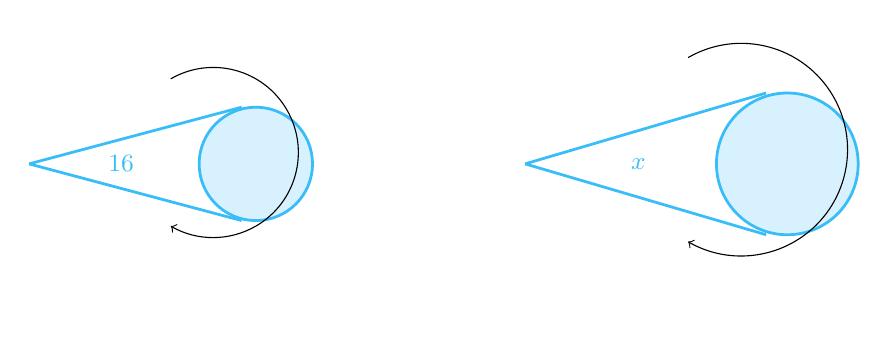
\begin{tikzpicture}[scale=0.9]
% smaller
\coordinate (V1) at (0,0);
\draw[shapeLine] (V1)--(3.0,0.8);
\draw[shapeLine] (V1)--(3.0,-0.8);
\draw[shapeFill] (3.2,0) circle (0.8);
\draw[->,dim] (2.0,1.2) arc (120:-120:1.2);
\node[dim] at (1.3,0) {$16$};
\node[lab] at (3.2,-1.6) {$A_1=120$};

% larger
\begin{scope}[xshift=7cm]
\coordinate (V2) at (0,0);
\draw[shapeLine] (V2)--(3.4,1.0);
\draw[shapeLine] (V2)--(3.4,-1.0);
\draw[shapeFill] (3.7,0) circle (1.0);
\draw[->,dim] (2.3,1.5) arc (120:-120:1.5);
\node[dim] at (1.6,0) {$x$};
\node[lab] at (3.7,-1.9) {$A_2=180$};
\end{scope}
\end{tikzpicture}
\end{center}

\tcblower
\textcolor{green}{\bfseries Answer:}
\[
\begin{aligned}
\Step{1}\;& \frac{A_2}{A_1}=\frac{180}{120}=\frac{3}{2}.\\
\Step{2}\;& k=\sqrt{\frac{3}{2}}=\frac{\sqrt{6}}{2}.\\
\Step{3}\;& x = 16\cdot \frac{\sqrt{6}}{2}=8\sqrt{6}\approx 19.6.
\end{aligned}
\]
\[
\boxed{x=8\sqrt{6}\text{ cm}\;(\approx 19.6\text{ cm})}
\]
\end{QAPair}

% ============================================================
% Q3
\begin{QAPair}{Question 3 (i)-(iii)}
\textcolor{gold}{\bfseries Question:} Radii of two spheres are $6$ cm and $8$ cm respectively. Find:\\
(i) ratio of areas of both spheres.\\
(ii) area of larger sphere if area of smaller sphere is $360\text{ cm}^2$.\\
(iii) area of smaller sphere if area of larger sphere is $1600\text{ cm}^2$.

\begin{center}
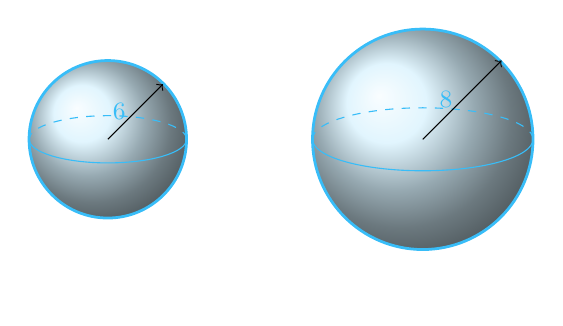
\begin{tikzpicture}
  \shade[ball color=cyan!20] (0,0) circle (1.0);
  \draw[shapeLine] (0,0) circle (1.0);
  \draw[cyan] (-1.0,0) arc (180:360:1.0 and 0.3);
  \draw[cyan, dashed] (1.0,0) arc (0:180:1.0 and 0.3);
  \draw[dim, ->] (0,0) -- (0.7,0.7) node[midway, left] {$6$};
  \node[lab, below] at (0,-1.1) {Small};

  \begin{scope}[xshift=4cm]
    \shade[ball color=cyan!20] (0,0) circle (1.4);
    \draw[shapeLine] (0,0) circle (1.4);
    \draw[cyan] (-1.4,0) arc (180:360:1.4 and 0.4);
    \draw[cyan, dashed] (1.4,0) arc (0:180:1.4 and 0.4);
    \draw[dim, ->] (0,0) -- (1.0,1.0) node[midway, left] {$8$};
    \node[lab, below] at (0,-1.5) {Large};
  \end{scope}
\end{tikzpicture}
\end{center}

\tcblower
\textcolor{green}{\bfseries Answer:}
\[
\begin{aligned}
\textbf{(i)}\;& \text{Ratio } = r_1^2 : r_2^2 = 6^2:8^2 = 36:64 = \mathbf{9:16}.\\
\textbf{(ii)}\;& A_{\text{large}} = 360 \times \frac{16}{9} = 40 \times 16 = \mathbf{640\text{ cm}^2}.\\
\textbf{(iii)}\;& A_{\text{small}} = 1600 \times \frac{9}{16} = 100 \times 9 = \mathbf{900\text{ cm}^2}.
\end{aligned}
\]
\end{QAPair}

% ============================================================
% Q4
\begin{QAPair}{Question 4}
\textcolor{gold}{\bfseries Question:} Ratio of areas of two regular pentagons is $16:25$.
Find ratio of their sides. Find side of second pentagon if side of first is $8$ cm.

\begin{center}
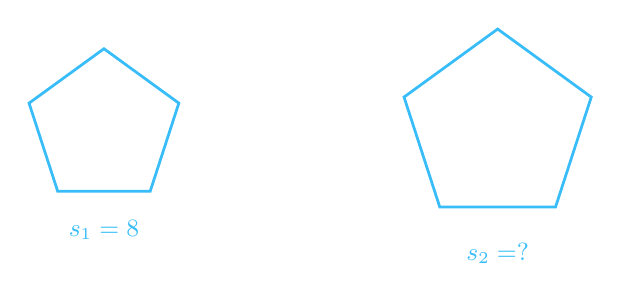
\begin{tikzpicture}
  \node[regular polygon, regular polygon sides=5, draw=cyan, line width=1pt, minimum size=2cm] (P1) at (0,0) {};
  \node[dim] at (0,-1.3) {$s_1=8$};
  \node[lab] at (0,0) {$A \propto 16$};

  \begin{scope}[xshift=5cm]
    \node[regular polygon, regular polygon sides=5, draw=cyan, line width=1pt, minimum size=2.5cm] (P2) at (0,0) {};
    \node[dim] at (0,-1.6) {$s_2=?$};
    \node[lab] at (0,0) {$A \propto 25$};
  \end{scope}
\end{tikzpicture}
\end{center}

\tcblower
\textcolor{green}{\bfseries Answer:}
\[
\begin{aligned}
\Step{1}\;& \text{Side ratio } = \sqrt{\text{Area ratio}} = \sqrt{\frac{16}{25}} = \frac{4}{5}.\\
\Step{2}\;& s_1:s_2 = \mathbf{4:5}.\\
\Step{3}\;& \frac{8}{s_2} = \frac{4}{5} \Rightarrow s_2 = 8 \times \frac{5}{4} = \mathbf{10\text{ cm}}.
\end{aligned}
\]
\end{QAPair}

% ============================================================
% Q5
\begin{QAPair}{Question 5}
\textcolor{gold}{\bfseries Question:} In the figure, $AB \parallel YZ$.
If areas of triangles $XAB$ and $XYZ$ are in the ratio $25:36$, find $\dfrac{XB}{XZ}$ and $\dfrac{AB}{YZ}$.
Are the ratios equal?

\begin{center}
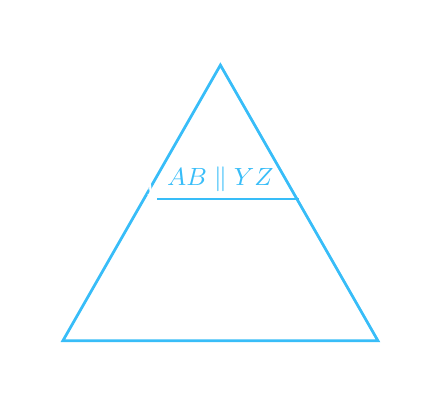
\begin{tikzpicture}[scale=1.0]
\coordinate (X) at (2,3.5);
\coordinate (Y) at (0,0);
\coordinate (Z) at (4,0);
\coordinate (A) at (1.2,1.8);
\coordinate (B) at (3.0,1.8);
\draw[shapeLine] (Y)--(X)--(Z)--cycle;
\draw[shapeLine] (A)--(B);
\node[lab] at (2,3.75) {$X$};
\node[lab] at (-0.2,-0.1) {$Y$};
\node[lab] at (4.2,-0.1) {$Z$};
\node[lab] at (1.05,1.95) {$A$};
\node[lab] at (3.15,1.95) {$B$};
\node[dim] at (2,2.05) {$AB\parallel YZ$};
\end{tikzpicture}
\end{center}

\tcblower
\textcolor{green}{\bfseries Answer:}
\[
\begin{aligned}
\Step{1}\;& AB\parallel YZ \Rightarrow \triangle XAB \sim \triangle XYZ.\\
\Step{2}\;& \frac{[XAB]}{[XYZ]}=\frac{25}{36}
=\left(\frac{XB}{XZ}\right)^2
=\left(\frac{AB}{YZ}\right)^2.\\
\Step{3}\;& \frac{XB}{XZ}=\sqrt{\frac{25}{36}}=\frac{5}{6},
\qquad
\frac{AB}{YZ}=\sqrt{\frac{25}{36}}=\frac{5}{6}.
\end{aligned}
\]
\[
\boxed{\frac{XB}{XZ}=\frac{5}{6}\;\;,\;\;\frac{AB}{YZ}=\frac{5}{6}\;\;\text{and they are equal.}}
\]
\end{QAPair}

% ============================================================
% Q6
\begin{QAPair}{Question 6}
\textcolor{gold}{\bfseries Question:} In a map, length of a $10$m wall is shown by $5$ cm.
If area of wall shown on the map is $1400\text{ cm}^2$, find the area of actual wall.

\begin{center}
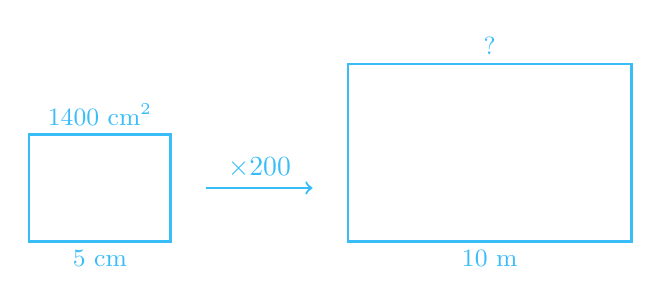
\begin{tikzpicture}[scale=0.9]
  % Map
  \draw[shapeLine] (0,0) rectangle (2,1.5);
  \node[lab] at (1,0.75) {Map};
  \node[dim, below] at (1,0) {$5$ cm};
  \node[dim, above] at (1,1.5) {$1400$ cm$^2$};

  % Arrow
  \draw[->, cyan, thick] (2.5,0.75) -- (4,0.75) node[midway, above] {$\times 200$};

  % Actual
  \begin{scope}[xshift=4.5cm]
    \draw[shapeLine] (0,0) rectangle (4,2.5);
    \node[lab] at (2,1.25) {Actual};
    \node[dim, below] at (2,0) {$10$ m};
    \node[dim, above] at (2,2.5) {$?$};
  \end{scope}
\end{tikzpicture}
\end{center}

\tcblower
\textcolor{green}{\bfseries Answer:}
\[
\begin{aligned}
\Step{1}\;& 10\text{ m} = 1000\text{ cm}.\\
\Step{2}\;& \text{Length scale } k = \frac{1000}{5}=200.\\
\Step{3}\;& \text{Area scale} = k^2 = 200^2 = 40000.\\
\Step{4}\;& A_{\text{actual}}=1400\times 40000=56{,}000{,}000\text{ cm}^2 = \mathbf{5600\text{ m}^2}.
\end{aligned}
\]
\end{QAPair}

% ============================================================
% Q7
\begin{QAPair}{Question 7 (i)-(ii)}
\textcolor{gold}{\bfseries Question:} Two cuboids are similar. Height of smaller cuboid is one-third of bigger one.
(i) Ratio of surface area of larger to smaller.
(ii) Surface area of bigger if smaller is $350\text{ cm}^2$.

\begin{center}
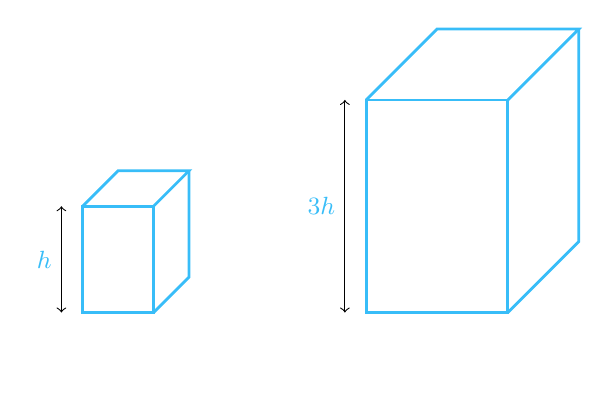
\begin{tikzpicture}[scale=0.9]
    % Small
    \draw[shapeLine] (0,0) rectangle (1,1.5);
    \draw[shapeLine] (0,1.5) -- (0.5,2.0) -- (1.5,2.0) -- (1,1.5);
    \draw[shapeLine] (1.5,2.0) -- (1.5,0.5) -- (1,0);
    \draw[dim, <->] (-0.3,0) -- (-0.3,1.5) node[midway, left] {$h$};
    \node[lab, below] at (0.5,-0.2) {Small};

    % Large
    \begin{scope}[xshift=4cm]
    \draw[shapeLine] (0,0) rectangle (2,3.0);
    \draw[shapeLine] (0,3.0) -- (1.0,4.0) -- (3.0,4.0) -- (2,3.0);
    \draw[shapeLine] (3.0,4.0) -- (3.0,1.0) -- (2,0);
    \draw[dim, <->] (-0.3,0) -- (-0.3,3.0) node[midway, left] {$3h$};
    \node[lab, below] at (1.5,-0.2) {Large};
    \end{scope}
\end{tikzpicture}
\end{center}

\tcblower
\textcolor{green}{\bfseries Answer:}
\[
\begin{aligned}
\textbf{(i)}\;& \text{Length ratio (Large:Small)} = 3:1.\\
&\text{Area ratio} = 3^2 : 1^2 = \mathbf{9:1}.\\
\textbf{(ii)}\;& A_{\text{big}} = 9 \times 350 = \mathbf{3150\text{ cm}^2}.
\end{aligned}
\]
\end{QAPair}

% ============================================================
% Q8
\begin{QAPair}{Question 8 (i)-(iv)}
\textcolor{gold}{\bfseries Question:} In the figure, $BC \parallel DE$. $AC=8$, $CE=5$. Find:
(i) $BC/DE$ and $AB/AD$. (ii) Area ratio. (iii) Area ABC if ADE is 507. (iv) Area BDEC.

\begin{center}
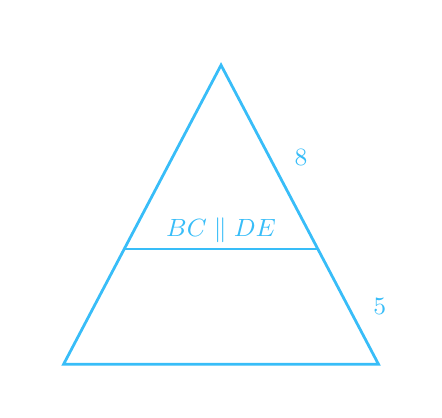
\begin{tikzpicture}[scale=1.0]
\coordinate (A) at (2,3.8);
\coordinate (D) at (0,0);
\coordinate (E) at (4,0);
% choose B and C on AD and AE with similarity ratio 8/13
\coordinate (B) at ($(A)!0.615!(D)$); 
\coordinate (C) at ($(A)!0.615!(E)$); 
\draw[shapeLine] (D)--(A)--(E)--cycle;
\draw[shapeLine] (B)--(C);
\node[lab] at (2,4.05) {$A$};
\node[lab] at (-0.2,-0.1) {$D$};
\node[lab] at (4.2,-0.1) {$E$};
\node[lab] at ($(B)+(-0.2,0.1)$) {$B$};
\node[lab] at ($(C)+(0.2,0.1)$) {$C$};
\node[dim] at (2,1.7) {$BC\parallel DE$};

% label AC and CE on right side
\draw[dim] ($(A)!0.50!(C)+(0.4,0)$) node {$8$};
\draw[dim] ($(C)!0.50!(E)+(0.4,0)$) node {$5$};
\end{tikzpicture}
\end{center}

\tcblower
\textcolor{green}{\bfseries Answer:}
\[
\begin{aligned}
\textbf{(i)}\;& AE=8+5=13. \quad \frac{BC}{DE}=\frac{AB}{AD}=\frac{AC}{AE}=\mathbf{\frac{8}{13}}.\\
\textbf{(ii)}\;& \frac{[ABC]}{[ADE]}=\left(\frac{8}{13}\right)^2=\mathbf{\frac{64}{169}}.\\
\textbf{(iii)}\;& [ABC]=507 \times \frac{64}{169} = 3 \times 64 = \mathbf{192\text{ cm}^2}.\\
\textbf{(iv)}\;& [BDEC]=507 - 192 = \mathbf{315\text{ cm}^2}. \quad (\text{Trapezium}).
\end{aligned}
\]
\end{QAPair}

\end{document}